\chapter{Ferramentas e Métodos}
\label{chap: ferramentas}

Esta seção visa descrever as ferramentas e os métodos utilizados para o desenvolvimento e a avaliação do algoritmo de Grover em dispositivos qu\^{a}nticos. Inicialmente, apresenta-se o uso de simuladores qu\^{a}nticos, em especial o AerSimulator, que permite a emulação de circuitos qu\^{a}nticos sob condições realistas de ruído, possibilitando uma análise mais próxima do comportamento esperado em hardware físico.

Em seguida, são detalhadas as características dos computadores qu\^{a}nticos utilizados nos testes, especificamente os \textit{backends} disponibilizados pela IBM Quantum. A escolha de múltiplos dispositivos com diferentes configurações visa proporcionar uma avaliação comparativa do desempenho do algoritmo em distintas arquiteturas e condições operacionais.

Por fim, é abordada a estrutura matemática e funcional do Algoritmo de Grover, descrevendo-se as principais etapas necessárias para sua implementação e destacando-se os conceitos fundamentais que sustentam sua eficiência em relação aos métodos clássicos de busca.

Esse conjunto de ferramentas e procedimentos estabelece a base metodológica para os experimentos realizados, permitindo uma análise abrangente dos resultados obtidos.
%
\section{Dispositivos Qu\^{a}nticos}
\label{sec: dispositivosQuanticos}

\subsection{Simuladores}
\label{subSec: simuladores}

Para avaliar o desempenho do algoritmo de Grover em condições que refletem as imperfeições de um dispositivo qu\^{a}ntico real, ser\'{a} utilizado o simulador \emph{AerSimulator} \cite{qiskit_aersimulator}, uma classe pertencente ao \emph{Qiskit Aer} \cite{qiskit_aer}, que, por sua vez, \'{e} um módulo do \emph{Qiskit}. Este simulador possibilita a emulaç\~{a}o de circuitos qu\^{a}nticos com a inclus\~{a}o de modelos de ruído específicos de cada QPU, proporcionando uma an\'{a}lise mais realista do algoritmo desenvolvido. Isso ocorre porque o \emph{AerSimulator} \'{e} capaz de reproduzir, de forma aproximada, o comportamento de dispositivos reais, previamente selecionados, permitindo avaliar o desempenho do algoritmo de Grover sob as limitações físicas e operacionais típicas do \textit{hardware} qu\^{a}ntico. Para fins de comparaç\~{a}o, ser\~{a}o utilizados os modelos de ruído correspondentes aos mesmos dispositivos qu\^{a}nticos (\textit{backends}) reais que, posteriormente, computar\~{a}o o algoritmo.

\subsection{Computadores}
\label{subSec: computadores}

Para realizar os testes, foram utilizados dois diferentes \textit{backends}: \href{https://quantum.cloud.ibm.com/computers?system=ibm_brisbane}{ibm\_brisbane} e \href{https://quantum.cloud.ibm.com/computers?system=ibm_torino}{ibm\_torino}. O \textit{ibm\_brisbane} é um processador baseado na tecnologia Eagle r3, com $127$ \textit{qubits} e conectividade otimizada para execução de circuitos de médio porte. Já o \textit{ibm\_torino} é um dispositivo mais recente, baseado na arquitetura Heron r1, com $133$ \textit{qubits} e melhorias no tempo de coerência e fidelidade de portas. Todos s\~{a}o de acesso livre atrav\'{e}s do serviço de computaç\~{a}o em nuvem IBM Quantum \cite{IBM_resources}.

Esses \textit{backends} correspondem a Processadores Qu\^{a}nticos (QPUs) supercondutores que operam com qubits físicos implementados por circuitos de transmon. A IBM disponibiliza informações detalhadas sobre cada um de seus dispositivos, incluindo a topologia de acoplamento, as portas qu\^{a}nticas nativas, bem como m\'{e}tricas importantes para a execuç\~{a}o de algoritmos, como tempos de coer\^{e}ncia ($T_1$  e $T_2$), fidelidades de operaç\~{a}o e taxas de erro de leitura \cite{IBM_backends}.

O uso desses \textit{backends} permite avaliar o desempenho do algoritmo de Grover n\~{a}o apenas em ambientes simulados, mas tamb\'{e}m em dispositivos físicos sujeitos a ruído real, decoer\^{e}ncia e demais limitações tecnológicas inerentes aos atuais computadores qu\^{a}nticos de uso geral \cite{Preskill2018_NISQ}. Al\'{e}m disso, cada \textit{backend} possui configurações distintas de conectividade entre qubits e diferentes níveis de fidelidade operacional, o que possibilita uma an\'{a}lise comparativa do impacto dessas vari\'{a}veis na execuç\~{a}o do algoritmo. O Quadro~\ref{tab: backends} mostra como exemplo, dois \textit{backends} disponíveis na \textit{IBM Quantum Platform}, e que serão utilizados tanto para simulações quanto para as execuções nas QPU's reais. 

\begin{quadro}[htb!]
  \begin{center}
    \caption{Configurações dos Computadores Qu\^{a}nticos utilizados} 
    \label{tab: backends}
    \vspace{0.2cm}
    \footnotesize
    \begin{tabular}{|lcccc|}
      \hline
      Backends & $\text{N}^\circ$ qubits & CLOPS & QPU & Portas Base \\
      % \hline
      \hline
      ibm\_brisbane & 127 & 180k & Eagle r3 & ECR, ID, RZ, SX, X \\
      ibm\_torino & 133 & 210k & Heron r1 & CZ, ID, RX, RZ, RZZ, SX, X \\
      \hline 
    \end{tabular}
  \end{center}
  \centering {\small Fonte: \cite{IBM_resources}} %Fonte do quadro
\end{quadro}

Nesse quadro pode-se analisar a quantidade de \textit{qubits} ($\text{N}^\circ$ qubits), o número de CLOPS\footnote{CLOPS é uma métrica criada pela IBM para medir quantas camadas de portas quânticas um processador consegue executar por segundo. Camadas, por sua vez, são as operações que podem ser executadas em paralelo, \textit{i. e.}, portas lógicas atuando em diferentes canais (\textit{qubits}) de forma independente podem ser executados ao mesmo tempo.} (\textit{Circuit Layer Operations Per Second}), o tipo de processador (QPU) e as portas base\footnote{Portas Base, ou \textit{basis gates}, representam o conjunto de operações nativas que um processador quântico consegue executar diretamente no \textit{hardware}, \textit{i. e.} as portas que não precisam ser reescritas no processo de compilação do circuito virtual para o físico.} de cada \textit{backend}.
\section{Visão Geral do Algoritmo de Grover}
\label{sec:algGroverGeral}

Como j\'{a} mencionado, o Algoritmo de Grover apresenta um m\'{e}todo de busca em listas que n\~{a}o possuem qualquer tipo de ordenaç\~{a}o com uma efici\^{e}ncia de ordem quadr\'{a}tica, por meio de uma t\'{e}cnica de amplificaç\~{a}o tanto de amplitudes quanto das probabilidades.
Seja a ilustraç\~{a}o apresentada na Figura~\ref{fig:itemMarcado},

\begin{figure}[ht!]
    \centering
    \caption{Lista com $2^{n}$ itens e um elemento $\omega$ marcado.}
    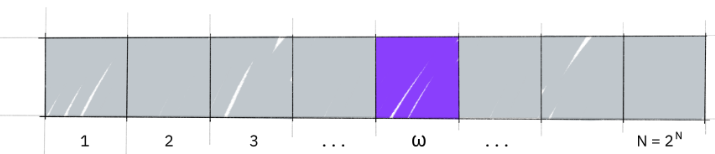
\includegraphics[scale=.6]{Imagens/markedItem.png}\\
    {\small Fonte: Github/\emph{Qiskit}}
    \label{fig:itemMarcado}
\end{figure}

Aqui tem-se ilustrado um conjunto contendo $N = 2^n$ elementos organizados aleatoriamente. Nele, h\'{a} um termo $\omega$ destacado, nomeado "\textit{winner}", que \'{e} justamente o elemento procurado. Se quisesse-se buscar o item marcado por meio de computaç\~{a}o cl\'{a}ssica, seriam necess\'{a}rias, em m\'{e}dia, $\frac{N}{2}$ iterações, contudo, ao implementarmos o Algoritmo de Grover, esse valor cai para $\sqrt{N}$, que \'{e} um avanço significativo, principalmente quando considera-se manipular conjuntos com grandes quantidades de itens \cite{qiskit_GroverNotebook}.

\subsection{Estrutura}
\label{subsec:estruturaAlg}

Para que seja poss\'{i}vel compreender a atuaç\~{a}o do algoritmo, \'{e} preciso entender sua estrutura, que conta com tr\^{e}s partes necess\'{a}rias para que possa ser implementado, sendo elas: preparaç\~{a}o inicial do estado, determinaç\~{a}o do Or\'{a}culo (marcaç\~{a}o do estado buscado) e amplificaç\~{a}o da amplitude e probabilidade (aplicaç\~{a}o do Operador de Grover ou Operador de Difus\~{a}o). Isso pode ser exemplificado pelo esquema da Figura~\ref{fig:groverEsquema}.

\begin{figure}[ht!]
    \centering
    % \captionsetup{justification=centering}
    \caption{Esquematizaç\~{a}o da estrutura do Algoritmo de Grover.}
    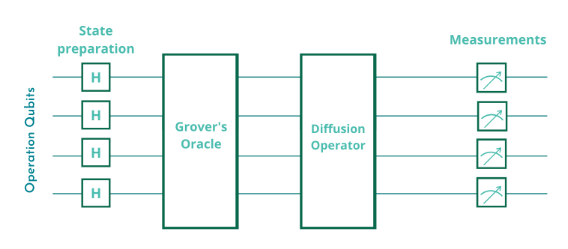
\includegraphics[width=.7\textwidth]{Imagens/esquemaG.png}\\
    {\small Fonte: Github/\emph{Qiskit}.}
    \label{fig:groverEsquema}
\end{figure}

Na preparaç\~{a}o do estado h\'{a} a criaç\~{a}o do que chamaremos de espaço de pesquisa, \'{e} o conjunto que cont\'{e}m o elemento marcado e onde ele ser\'{a} procurado. 

Feito isso, seguiremos para a determinaç\~{a}o do item que queremos encontrar, que \'{e} feita pelo Or\'{a}culo. A atuaç\~{a}o do Or\'{a}culo consiste em inverter a fase do elemento de interesse, ou seja, ele marca o item buscado. Caso haja mais de um item de interesse, o Or\'{a}culo deve agir em todos eles, marcando-os, de modo que sejam destacados pelo difusor.

Por fim, utiliza-se o Operador de Difus\~{a}o para aumentar a amplitude do estado marcado, enquanto decresce as demais, sendo assim uma garantia de que na medida final, o resultado obtido seja aquele procurado.

% \subsection{Funcionamento}
% \label{subsec:funcionamentoAlg}
Quando trabalha-se com o Algoritmo de Grover, pode-se reduzir o problema a um espaço de duas dimensões, sendo necess\'{a}rio considerar apenas o estado buscado -- \textit{winner}, $\ket{\omega}$ --, e a superposiç\~{a}o uniforme, $\ket{s}$. Contudo, esses n\~{a}o s\~{a}o vetores perpendiculares entre si, uma vez que $\ket{\omega}$ ocorre em superposiç\~{a}o com amplitude $\frac{1}{\sqrt{N}}$. Para contornar isso, cria-se um vetor $\ket{s'}$ que \'{e} perpendicular a $\ket{\omega}$, formando assim o plano bidimensional apresentado na Figura~\ref{subfig:Plano}. Na Figura~\ref{subfig:Amplitude}, est\~{a}o ilustradas as amplitudes dos itens contidos no conjunto, evidenciando o elemento \textit{winner}.

\begin{figure}[ht!]
    \centering
    \caption{Plano Bidimensional e Amplitude dos estados da base.}
    \label{fig:espacoAmplitude}
    \begin{subfigure}[b]{0.4\textwidth}
        \centering
        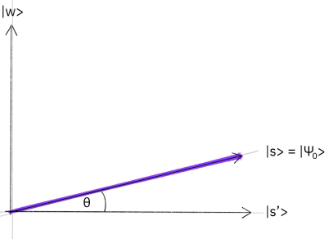
\includegraphics[width=\textwidth]{Imagens/BidimensionalEspaco.png}
        \caption{Plano formado pelos vetores $\ket{\omega}$ e $\ket{s'}$.}
        \label{subfig:Plano}
    \end{subfigure}
    \hfill
    \begin{subfigure}[b]{0.45\textwidth}
        \centering
        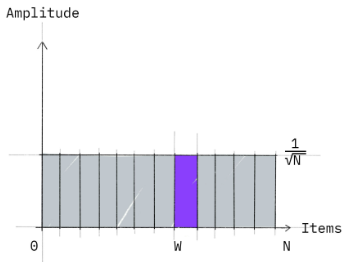
\includegraphics[width=\textwidth]{Imagens/AmplitudesW.png}
        \caption{Amplitude dos itens do conjunto, com $\ket{\omega}$ em destaque.}
        \label{subfig:Amplitude}
    \end{subfigure}

    \vspace{0.3em}
    {\small Fonte: Github/\emph{Qiskit}.}
\end{figure}


% Uma vez introduzida a vis\~{a}o geral sobre como o algoritmo atua, pode-se passar para o estudo de cada uma de suas tr\^{e}s etapas.

%%%%%%%%%%%%%%%%%%%%%%%%%%%%%%%%%%%%%%%%%%%%%%%%%%%%%%%%%%%%%%%%%%%%%%%%%%%%%%%%%%

\subsection{Preparaç\~{a}o Inicial}
\label{subsec:prepInicialAlg}

A Preparaç\~{a}o Inicial \'{e} a etapa inicial do algoritmo, na qual o Espaço de Pesquisa \'{e} criado, matematicamente descrito como uma superposiç\~{a}o uniforme e pela Equaç\~{a}o~\ref{eq:superposicao}, e possui tamanho dado por $N = 2^n$, com $n$ sendo o n\'{u}mero de qubits.

\begin{equation}
    \ket{s} = \frac{1}{\sqrt{N}}\sum_{x = 0}^{N - 1} \ket{bin(x)},
    \label{eq:superposicao}
\end{equation}
%
com $x \in \left\{ 0, 1, 2, \ldots, N-1 \right\}$.

Se uma mediç\~{a}o for realizada na base $\ket{x}$, de acordo com o Quinto Postulado da Mec\^{a}nica Qu\^{a}ntica \cite{vonNuemann1955_QuMec}, a superposiç\~{a}o colapsa, podendo resultar em qualquer um dos estados de mesma probabilidade $\frac{1}{N} = \frac{1}{2^n}$. 

Em termos de circuito qu\^{a}ntico, a superposiç\~{a}o explicitada pela Equaç\~{a}o~\ref{eq:superposicao} pode ser constru\'{i}da facilmente aplicando a porta Hadamard em cada um dos qubits, que se iniciam no estado fundamental $\ket{0}$, como representado pela Equaç\~{a}o~\ref{eq:preparacaoInicial}.
%
\begin{equation}
    \ket{s} = H^{\otimes n}~\ket{0}^n
    \label{eq:preparacaoInicial}
\end{equation}

O vetor $\ket{s}$ que aparece na Figura~\ref{subfig:Plano} pode ser escrito em coordenadas polares, como
%
\begin{equation}
    \ket{s} = \sin{\theta}\ket{\omega} + \cos{\theta}\ket{s'},
    \label{eq:estadoCoordPolar}
\end{equation}

em que 
%
\begin{equation}
    \theta = \arcsin{\braket{s|\omega}} = \arcsin{\frac{1}{\sqrt{N}}}
    \label{eq:thetaValue}
\end{equation}

\subsection{Or\'{a}culo ($U_f$)}
\label{subsec:oraculoAlg}

Tomando a premissa de que o elemento $\omega$ procurado está em um determinado conjunto contendo $N = 2^n$ itens, ${0, 1, 2, ..., N-1}$, com $n \in \mathbb{N}$, podemos recorrer a uma função $f : {0, 1, 2, ..., N-1},\\ \to {1,-1}$ que atua na amplitude dos elementos para marcar o buscado, sendo $f$ tal que
%
\begin{equation}
    f(x) = 
    \begin{cases}
        -1, & \text{se } x = \omega \\
        1, & \text{se } x \neq \omega
    \end{cases}
    \label{eq:fx Oraculo}
\end{equation}

Em outras palavras, o Oráculo, denotado por \simboloinline{$U_f$}{Operador Oráculo}, nada mais é que uma função que gera a reflexão em um \^{a}ngulo $\theta$ de $\ket{s}$ sobre $\ket{s'}$, bem como a reflexão da amplitude do elemento de interesse $\ket{\omega}$, que pode ser visualizado com a ajuda da Figura~\ref{fig:rotacaoReflexao}.

\begin{figure}[ht!]
    \centering
    \captionsetup{justification=centering}
    \caption{Reflexão dos estados $\ket{s}$ e $\ket{\omega}$, respectivamente.}

    \begin{subfigure}[b]{0.4\textwidth}
        \centering
        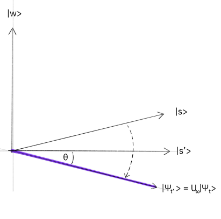
\includegraphics[width=\textwidth]{Imagens/rotacao.png}
        \caption{Reflexão de $\ket{s}$ sobre $\ket{s'}$ em um \^{a}ngulo $\theta$.}
        \label{subfig:rotacao}
    \end{subfigure}
    \hfill
    \begin{subfigure}[b]{0.45\textwidth}
        \centering
        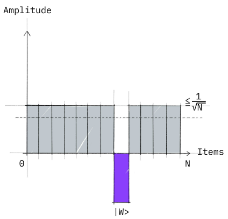
\includegraphics[width=\textwidth]{Imagens/reflexao.png}
        \caption{Reflexão de $\pi$ rads na amplitude de $\ket{\omega}$.}
        \label{subfig:reflexao}
    \end{subfigure}

    \vspace{0.5em}
    {\small Fonte: Github/\emph{Qiskit}.}
    \label{fig:rotacaoReflexao}
\end{figure}


De modo geral, a construção dos Oráculos no Algoritmo de Grover pode ser realizada utilizando portas lógicas qu\^{a}nticas do tipo $X$ e \simboloinline{$MCZ$}{\textit{Porta Lógica Quântica Z-multi-controlada}}, seguindo a seguinte regra de formação:

\begin{enumerate}
\label{enum: regraFormacaoOraculo}
    \item Para cada qubit cujo valor no estado buscado seja $\ket{0}$, aplica-se uma porta $X$ nesse qubit, realizando assim um \textit{bit-flip};
    
    \item Em seguida, aplica-se uma porta ($MCZ$) sobre todos os qubits, marcando o estado desejado com um fator de fase;
    
    \item Por fim, aplica-se novamente a porta $X$ nos mesmos qubits que sofreram o \textit{bit-flip} na primeira etapa, revertendo as alterações realizadas inicialmente.
\end{enumerate}

\subsection{Operador de Difus\~{a}o ($U_s$)}
\label{subsec:difusaoAlg}

A  aplicação do Operador de Difusão, denotado por \simboloinline{$U_s$}{\textit{Operador de Difus\~{a}o}}, consiste em operações de amplificação sobre o estado $\ket{s}$, gerando uma reflexão adicional do mesmo.
%
\begin{equation}
    U_s = 2~\ket{s}\bra{s} - I
    \label{eq:Us}
\end{equation}

Essa transformação mapeia o estado de $\ket{s}$ para $(U_sU_f)\ket{s}$ e completa a transformação, tal como está apresentado na Figura~\ref{fig:transformacaoCompleta}.

\begin{figure}[ht!]
    \centering
    \captionsetup{justification=centering}
    \caption{Segunda reflexão dos estados $\ket{s}$ e $\ket{\omega}$, respectivamente.}
    \label{fig:transformacaoCompleta}  % Label principal após caption

    \begin{subfigure}[b]{0.4\textwidth}
        \centering
        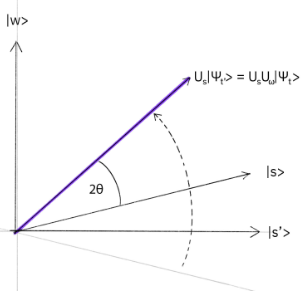
\includegraphics[width=\textwidth]{Imagens/reflexaoEstado.png}
        \caption{Segunda reflexão de $\ket{s}$ sobre $\ket{s'}$.}
        \label{subfig:reflexaoEstado}
    \end{subfigure}
    \hfill
    \begin{subfigure}[b]{0.48\textwidth}
        \centering
        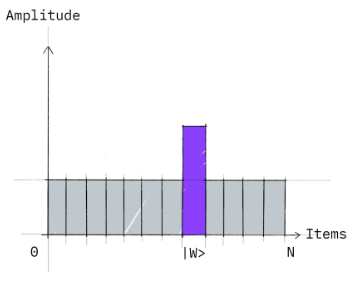
\includegraphics[width=\textwidth]{Imagens/reflexaoAmplitude.png}
        \caption{Segunda reflexão na amplitude de $\ket{\omega}$.}
        \label{subfig:reflexaoAmplitude}
    \end{subfigure}

    \vspace{0.5em}
    {\small Fonte: Github/\emph{Qiskit}.}
\end{figure}

Duas reflexões sempre resultam em uma rotação, que leva o estado inicial $\ket{s}$ para mais perto do elemento \textit{winner}, $\ket{\omega}$. 

Como esta é uma reflexão sobre $\ket{s}$, busca-se adicionar uma fase negativa a cada estado ortogonal a $\ket{s}$. A maneira como pode-se fazer isso é aplicar uma transforma\~{a}o que leva o estado $\ket{s} \to \ket{0}$, com isso, em vez de $U_s$, chamar-se-á $U_0$. Dessa forma, a Equaç\~{a}o~\ref{eq:Us} se torna: 
%
\begin{equation}
    U_0 = 2~\ket{0}\bra{0} - I
    \label{eq:Uo}
\end{equation}

Essa operação aplica uma fase negativa a todos os estados ortonormais a $\ket{0}$, como será demonstrado.

[TALVEZ COLOCAR NUM APÊNDICE***]

Aplicação do Operador $U_0$ em $\ket{s}$, com $\ket{s}$ podendo ser um conjunto arbitr\'{a}rio com $N-1$ itens:

\begin{equation*}
U_0~\ket{s} = \left(2\ket{0}\bra{0} - I\right) \frac{1}{\sqrt{N}}\sum_{x=0}^{N-1} \ket{bin(x)},
\end{equation*}

Expandindo, tem-se:

\begin{equation*}
2~\ket{0}\bra{0} \left( \frac{1}{\sqrt{N}}\sum_{x=0}^{N-1} \ket{bin(x)}\right) = \frac{1}{\sqrt{N}}\sum_{x=0}^{N-1} \ket{bin(x)}
\end{equation*}

\begin{equation}
2~\ket{0} \left( \sum_{x=0}^{15} \braket{0|bin(x)}\right) = \sum_{x=0}^{15} \ket{bin(x)}
\label{eq:aplicacaoDifusor 2}
\end{equation}
%
Como $\braket{0|bin(x)} = 1$ apenas se $x = 0$ (enquanto todos os outros termos se tornam $0$),  o único termo que sobrevive é:
%
\begin{equation*}
2\ket{0}{\braket{0|bin(0)}} = 2\ket{bin(0)}
\end{equation*}

Então, em síntese, tem-se:
%
\begin{align}
\notag
U_0~\ket{s} = &2~\ket{bin(0)} - \sum_{x=0}^{N-1} \ket{bin(x)} \\ 
\notag
= &2~\ket{bin(0)} - \ket{bin(0)} - \ket{bin(1)} - \ket{bin(2)} - \dots - \ket{bin(N-1)} \\ 
= &\ket{bin(0)} - \sum_{x=1}^{N-1} \ket{bin(x)}
\label{eq:aplicacaoDifusao}
\end{align}
%
Ou seja, a amplitude $\ket{bin(0)}$ aumenta em relação aos demais que invertem.

Tendo sido demonstrada a forma matemática, passa-se agora para a apresentação da obtenção do circuito qu\^{a}ntico que realiza essa operação. 

O Operador de Difusão em termos de portas lógicas é dado por:
%
\begin{equation}
    U_s = H^{\otimes n}~U_0~H^{\otimes n}
    \label{gate: operadorDifusao}
\end{equation}

Como já visto, a atuação de $U_0$ é aplicar uma fase negativa a todos os estados ortogonais a $\ket{s}$, e, para isso, deve ser realizada a seguinte sequência:

\begin{enumerate}
\label{enum: difusor}
    \item Aplicação de portas $X$ em todos canais para \textit{bit-flip} dos estados;
    \[\ket{00\cdots0} \to \ket{11\cdots1} \]
    \item Aplicação de porta $MCZ$, com alvo no último canal, pois dessa forma o último estado recebe uma inversão de fase;
    \begin{equation}
    MCZ_{[N \times N]}  =
    \begin{bmatrix}
        1 & 0 &  \cdots  & 0\\
        0 & 1 &  \cdots  & 0\\
        \vdots & \vdots & \ddots & \vdots \\
        0 & 0 &  \cdots & -1\\
    \end{bmatrix}_{[N \times N]}
    \label{mtx: gateMCZ}
\end{equation}
    \item Novamente aplica-se portas $X$ para desfazer os \textit{bit-flips}.
    \[\ket{11\cdots1} \to \ket{00\cdots0} \]
\end{enumerate}

Após a última etapa, o resultado obtido é:

\begin{equation*}
    \begin{bmatrix}
        -1 & 0 &  \cdots  & 0\\
        0 & 1 &  \cdots  & 0\\
        \vdots & \vdots & \ddots & \vdots \\
        0 & 0 &  \cdots & 1\\
    \end{bmatrix}_{[N \times N]}
\end{equation*}

Ou seja, existe ainda uma fase global em $U_0$, de modo que o Operador de Difusão, em termos de portas lógicas, é:
\begin{equation}
    U_0 = -X^{\otimes n}~MCZ~X^{\otimes n}
    \label{gate: difusor}
\end{equation}

O trecho de circuito descrito em Equação está mostrado na Figura~\ref{fig:difusor}

\begin{figure}[!htb]
\centering
\caption{Operador de Difus\~{a}o parcial}
\label{fig:difusor} 
\begin{quantikz}
\lstick{$q_0$}       & \gate{X} & \qw      & \ctrl{1}   & \qw       & \gate{X}  & \qw \\
\lstick{$q_1$}       & \gate{X} & \qw      & \ctrl{2}   & \qw       & \gate{X}  & \qw \\
\lstick{$\vdots$}    &~\vdots~  &          &            & \qw       &~\vdots~   & \qw \\
\lstick{$q_{n-1}$}   & \gate{X} & \gate{H} & \gate{X}   & \gate{H}  & \gate{X}  & \qw \\
\lstick{$c: n$}      & \cw      & \cw      & \cw        & \cw       & \cw       & \cw
\end{quantikz}

\vspace{.3em}
{\small Fonte: do autor} 
\end{figure}

Considerando as Equações~\ref{gate: operadorDifusao} e~\ref{gate: difusor}. Tem-se que o Operador de Difusão completo em portas lógicas qu\^{a}nticas são dados pela Equação~\ref{gate: operadorDifusaoCompleto} e pela Figura~\ref{fig:operadorDifusaoCompleto}.

\begin{equation}
    U_s = H^{\otimes n}~X^{\otimes n}~MCZ~X^{\otimes n}~H^{\otimes n}
    \label{gate: operadorDifusaoCompleto}
\end{equation}

Note que a fase negativa não foi acrescentada, pois não precisa ser considerada no circuito qu\^{a}ntico. 

\begin{figure}[!htb]
\centering
\caption{Operador de Difus\~{a}o completo}
\label{fig:operadorDifusaoCompleto} %rotulo para refencia
\begin{quantikz}
\lstick{$q_0$}       & \gate{H} & \gate{X} &          & \ctrl{1} &          & \gate{X} & \gate{H} & \qw \\
\lstick{$q_1$}       & \gate{H} & \gate{X} &          & \ctrl{2} &          & \gate{X} & \gate{H} & \qw \\
\lstick{$\vdots$}    &~\vdots~  &~\vdots~  &          &          &          & ~\vdots~ & ~\vdots~ & \qw \\
\lstick{$q_{n-1}$}   & \gate{H} & \gate{X} & \gate{H} & \gate{X} & \gate{H} & \gate{X} & \gate{H} & \qw \\
\lstick{$c: n$}      & \cw      & \cw      & \cw      & \cw      & \cw      & \cw      & \cw      & \cw
\end{quantikz}

\vspace{.3em}
{\small Fonte: do autor} 
\end{figure}

\subsection{Fator de Otimizac\~{a}o (k)}
\label{subsec:otimizacao k}

Afim de otimizar o resultado, a aplicação do \nameref{subsec:oraculoAlg} e do \nameref{subsec:difusaoAlg} deverão ser executados um número \simboloinline{$k$}{Fator de Otimização do Algoritmo de Grover} de vezes para que o resultado obtido seja o mais próximo possível (com maiores amplitudes e probabilidades) do estado esperado $\ket{\omega}$, e pode ser expresso por
%
\begin{equation}
    \label{eq:psi k}
    \ket{\psi_k} = (U_sU_f)^k\ket{s}
\end{equation}

O número ideal $k$ de iterações necessárias para que $\ket{\omega}$ seja obtido é dado por

\begin{equation}
    k = \frac{\pi}{4}\sqrt{\frac{N}{m}}
    \label{eq:k value}
\end{equation}
%
em que $N$ é o tamanho do espaço de pesquisa, e $m$ é a quantidade de itens procurados.

A Figura~\ref{fig:algoritmoCompleto} mostra um esquema do Algoritmo de Grover completo, evidenciando o Oráculo e o Operador de Difusão.

\begin{figure}[ht!]
    \centering
    \captionsetup{justification=centering}
    \caption{Esquematização do Algoritmo de Grover.}
    \label{fig:algoritmoCompleto}
    
    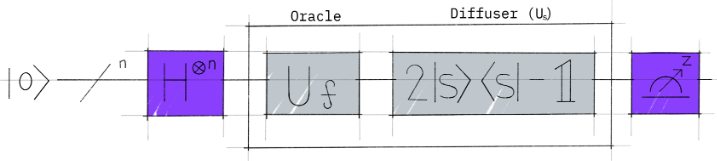
\includegraphics[scale=.5]{Imagens/esquemaAlgG.png}
    
    {\small Fonte: Github/\emph{Qiskit}.}
\end{figure}


